%% This is an example first chapter.  You should put chapter/appendix that you
%% write into a separate file, and add a line \include{yourfilename} to
%% main.tex, where `yourfilename.tex' is the name of the chapter/appendix file.
%% You can process specific files by typing their names in at the 
%% \files=
%% prompt when you run the file main.tex through LaTeX.

\singlespacing{

\chapter{Simulation Methods: Finite Difference, Finite Element, Finite Volume}

A differential equation is mathematical relationship between a function and at least one of its derivatives. For example:

 \begin{equation}\label{eq:diffEq}
 \frac{\partial^{2}f(x)}{\partial x^{2}} = f(x)
  \end{equation}
  \\
Equation \ref{eq:diffEq} describes a function $f$ with one independent variable $x$ using both the second order form $ \frac{\partial^{2}f(x)}{\partial x^{2}} $ and the zeroth order form $f(x)$.  Differential equations of single variable functions like equation \ref{eq:diffEq} are called \textit{ordinary differential equations} (ODE).  By contrast, a \textit{partial differential equation} (PDE) is a differential equation that describes multivariable functions, like $f(t, x, y)$.\\

A \textit{solution} to a differential equation is a function, $f$, that satisfies the differential relationship described by the differential equation.  This chapter covers methods of solving PDEs numerically, usually with the help of a computer.

\section{PDEs from Physics}

PDEs are common in physics as many physical phenomena are dynamic in both space and time.  In this section, I'll introduce some PDEs from physics and show how to solve them later in the chapter.

\subsubsection{Heat Equation}

The \href{https://en.wikipedia.org/wiki/Heat_equation}{heat equation} describes the dissipation of heat through materials:

 \begin{equation}\label{eq:heatEq}
 \frac{\partial T}{\partial t} = c\nabla^{2}T
   \end{equation}
     \\
    where $t$ is time, $T$ is the temperature, $c$ is a constant, and $\nabla^{2}$ is the sum of the partial derivatives of $u$ with respect to the spatial dimensions of $u$ (also called the spatial \href{https://en.wikipedia.org/wiki/Laplace_operator}{Laplacian}).\\
    
    The heat equation contains a first derivative of $u$ with respect to $t$ and a second derivative of $u$ with respect to the spatial dimensions.  PDEs are classified based on the highest order derivative they contain, so the heat equation is a second order PDE.\\
    
     We can write a version of the heat equation for 1D(\ref{eq:heat1d}), 2D(\ref{eq:heat2d}), or 3D(\ref{eq:heat3d}) by expanding the Laplacian appropriately:
 
 \begin{equation}\label{eq:heat1d}
  \frac{\partial T}{\partial t} = c\frac{\partial^{2}T}{\partial x^{2}}
  \end{equation}
  
   \begin{equation}\label{eq:heat2d}
  \frac{\partial T}{\partial t} = c\left(\frac{\partial^{2}T}{\partial x^{2}}+\frac{\partial^{2}T}{\partial y^{2}}\right)
  \end{equation}
  
   \begin{equation}\label{eq:heat3d}
  \frac{\partial T}{ \partial t} = c\left(\frac{\partial^{2}T}{\partial x^{2}}+\frac{\partial^{2}T}{\partial y^{2}}+\frac{\partial^{2}T}{\partial z^{2}} \right)
  \end{equation}
  
\subsubsection{Wave Equation}

 The \href{https://en.wikipedia.org/wiki/Wave_equation}{wave equation} shows up often in physics - electricity and magnetism, acoustics, fluid dynamics, solid mechanics, etc.  It describes the propagation of waves through space and bears close resemblance to the heat equation:

 \begin{equation}\label{eq:waveEq}
 \frac{\partial^{2}u}{\partial t^{2}} = c\nabla^{2}u
   \end{equation}
     \\
 where $t$ is time, $u$ is the amplitude of the wave, $c$ is a constant, and $\nabla^{2}$ is the spatial Laplacian.  Like the heat equation (\ref{eq:heatEq}), this PDE is second order because it involves the second derivative of $u$ with respect to both $t$ and the spatial dimensions. \\
 
The 1D(\ref{eq:wave1d}), 2D(\ref{eq:wave2d}), or 3D(\ref{eq:wave3d}) expansions of the wave equation are given below:
 
 \begin{equation}\label{eq:wave1d}
  \frac{\partial^{2}u}{\partial t^{2}} = c\frac{\partial^{2}u}{\partial x^{2}}
  \end{equation}
  
   \begin{equation}\label{eq:wave2d}
  \frac{\partial^{2}u}{\partial t^{2}} = c\left(\frac{\partial^{2}u}{\partial x^{2}}+\frac{\partial^{2}u}{\partial y^{2}}\right)
  \end{equation}
  
   \begin{equation}\label{eq:wave3d}
  \frac{\partial^{2}u}{ \partial t^{2}} = c\left(\frac{\partial^{2}u}{\partial x^{2}}+\frac{\partial^{2}u}{\partial y^{2}}+\frac{\partial^{2}u}{\partial z^{2}} \right)
  \end{equation}
    
  \subsubsection{Advection Equation}
  
  The \href{https://en.wikipedia.org/wiki/Advection}{advection equation} describes the transport of material by a fluid, such as silt in a river:
  
   \begin{equation}\label{eq:advection}
  \frac{\partial \psi}{\partial t} = -v \cdot \nabla\psi
  \end{equation}
   \\
    where $t$ is time, $\psi$ is the magnitude of advection, $v$ is the velocity field (a vector field), and $\nabla$ is the spatial gradient operator del.  since there are no second order or higher derivates present, equation \ref{eq:advection} is a first order PDE.\\
    
    Again, the 1D(\ref{eq:advection1d}), 2D(\ref{eq:advection2d}), or 3D(\ref{eq:advection3d}) expansions of the advection equation are given below:
 
 \begin{equation}\label{eq:advection1d}
  \frac{\partial \psi}{\partial t} = -v_{x}\frac{\partial \psi}{\partial x}
  \end{equation}
  
   \begin{equation}\label{eq:advection2d}
  \frac{\partial \psi}{\partial t} = -v_{x}\frac{\partial \psi}{\partial x}-v_{y}\frac{\partial \psi}{\partial y}
  \end{equation}
  
   \begin{equation}\label{eq:advection3d}
  \frac{\partial \psi}{\partial t} = -v_{x}\frac{\partial \psi}{\partial x}-v_{y}\frac{\partial \psi}{\partial y}-v_{z}\frac{\partial \psi}{\partial z}
  \end{equation}
  
\section{Analytical vs Numerical Solutions}

Sometimes it's possible to identify a continuous function that satisfies the relationships described by a differential equation; this is refereed to as a \textit{closed-form} solution or \textit{analytical} solution.  For example, $f(x)=e^{x}$ is an analytical solution to equation \ref{eq:diffEq}.  Usually, analytical solutions are the preferred form of the solution as they return exact values.\\

However, it is usually not possible to solve a PDE analytically, in these cases we must use numerical techniques to approximate the solution.  Generally, this involves splitting up, or \textit{discretizing}, space into a finite number of regions and evaluating the PDE in each of these regions.  Often this process of discretization is applied to time as well, creating a solution that moves forward in quantized time steps.  As the size of the spatial regions and temporal steps becomes very small, the discrete solution approaches the continuous, analytical solution to the PDE.

\section{Finite Difference Method}

The Finite Difference Method (FDM) assumes that space is broken up into identically sized regions on a grid (Fig \ref{fig:FDMGrid}) called \textit{differential elements}.  The size of the differential elements depends on the resolution of the grid.  For a 1D model, each element has length $\Delta x$., in a 2D model each element has one side of length $\Delta x$ and one side of length $\Delta y$, and so on.  Using equations called \textit{finite difference approximations}, it is possible to transform a PDE into a form that relates differential elements to their neighbors and solve for their states over time.\\

\begin{figure}
  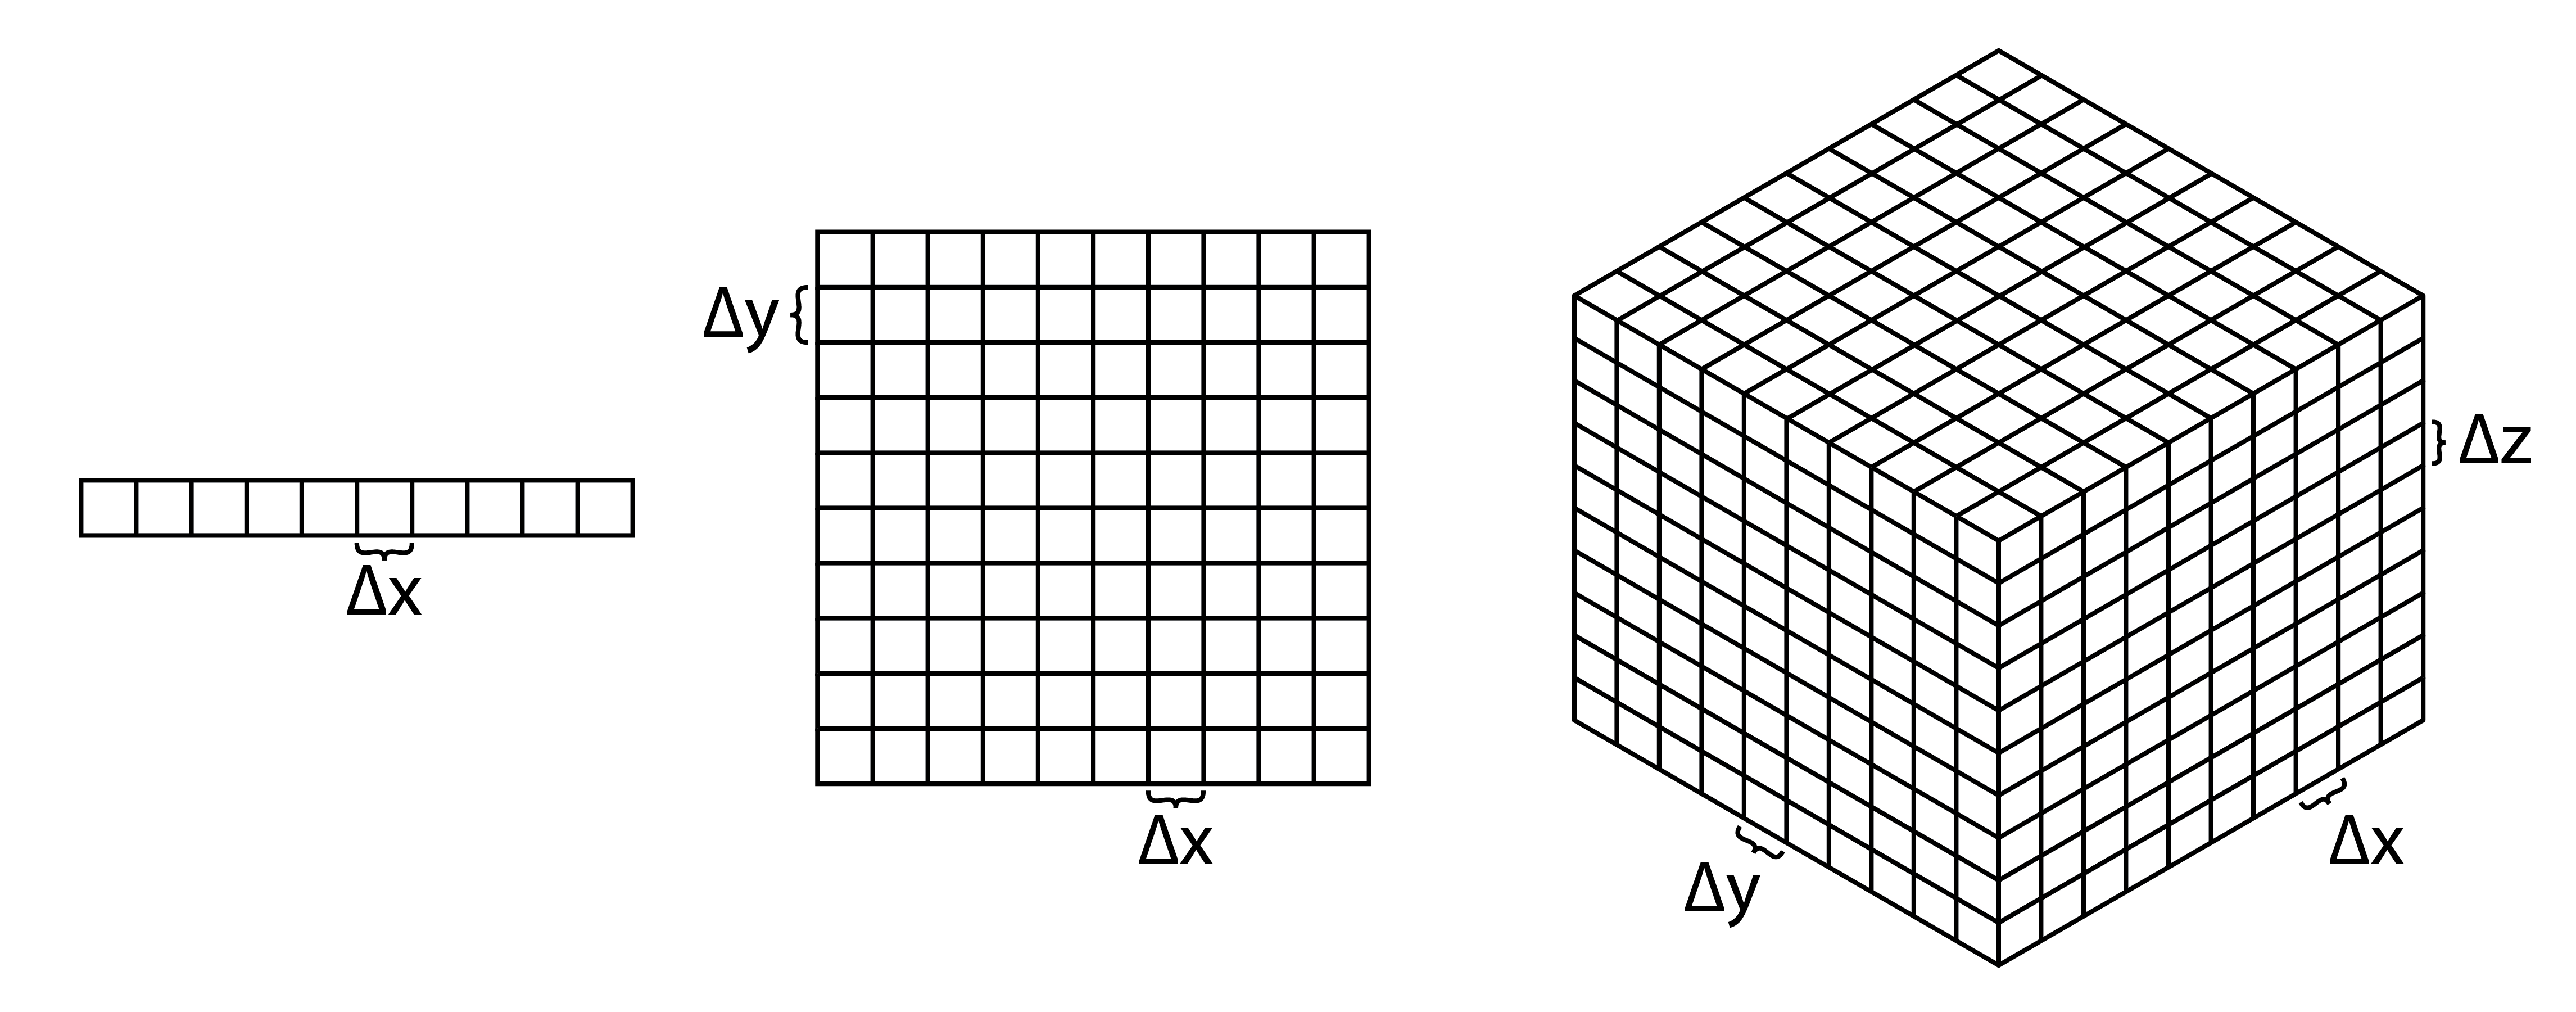
\includegraphics[width=\linewidth]{SimMethodsFDMGrid.png}
  \caption{FDM grids for 1D (right), 2D (middle) and 3D (left).}
  \label{fig:FDMGrid}
\end{figure}

A derivation of the finite difference approximations comes from the \href{https://en.wikipedia.org/wiki/Taylor_series}{Taylor Series}.  Imagine a continuous, differentiable function $f(x)$.  If we know some $f(x_{0})$, we can estimate $f(x_{0}+\Delta  x)$ with the Taylor Series expansion.  The n degree Taylor Series expansion around $f(x_{0})$ is given by:

 \begin{equation}\label{eq:norderTaylor}
  f(x_{0} + \Delta  x) = f(x_{0}) + \frac{f'(x_{0})}{1!}\Delta  x + \frac{f''(x_{0})}{2!}\Delta  x^{2} + \cdots  + \frac{f^{(n)}(x_{0})}{n!}\Delta  x^{n} + R_{n}(x_{0})
  \end{equation}
    \\
  where $f^{(n)}(x_{0})$ is the $n$th derivative of $f(x)$ with respect to $x$ evaluated at $x_{0}$, and $R_{n}(x_{0})$ is a remainder error term that depends on the degree of the Taylor expansion.  The Taylor expansion is not an approximation, it returns the exact value of $ f(x_{0} + \Delta  x)$; as $n$ approaches infinity, $R_{n}(x_{0})$ vanishes.\\

\subsection{First Order FDM}

A first order Taylor expansion reduces \ref{eq:norderTaylor} to:
  
 \begin{equation}\label{eq:1degTaylor}
  f(x_{0} + \Delta  x) = f(x_{0}) + f'(x_{0})\Delta x + R_{1}(x_{0})
  \end{equation}
    \\
  For small $\Delta  x$ it is OK to ignore the error term.  We are left with a first order Taylor \textit{approximation}:
  
   \begin{equation}\label{eq:1degTaylorApprox}
  f(x_{0} + \Delta  x) \approx f(x_{0}) + f'(x_{0})\Delta x
  \end{equation}
    \\
This is the same as tracing the slope of $f$ at $x_{0}$ to approximate a nearby value (Fig \ref{fig:FDMSlopeApprox}).  Rearranging \ref{eq:1degTaylorApprox} gives us an expression for the first derivative of $f(x)$ with respect to $x$:

\begin{figure}
  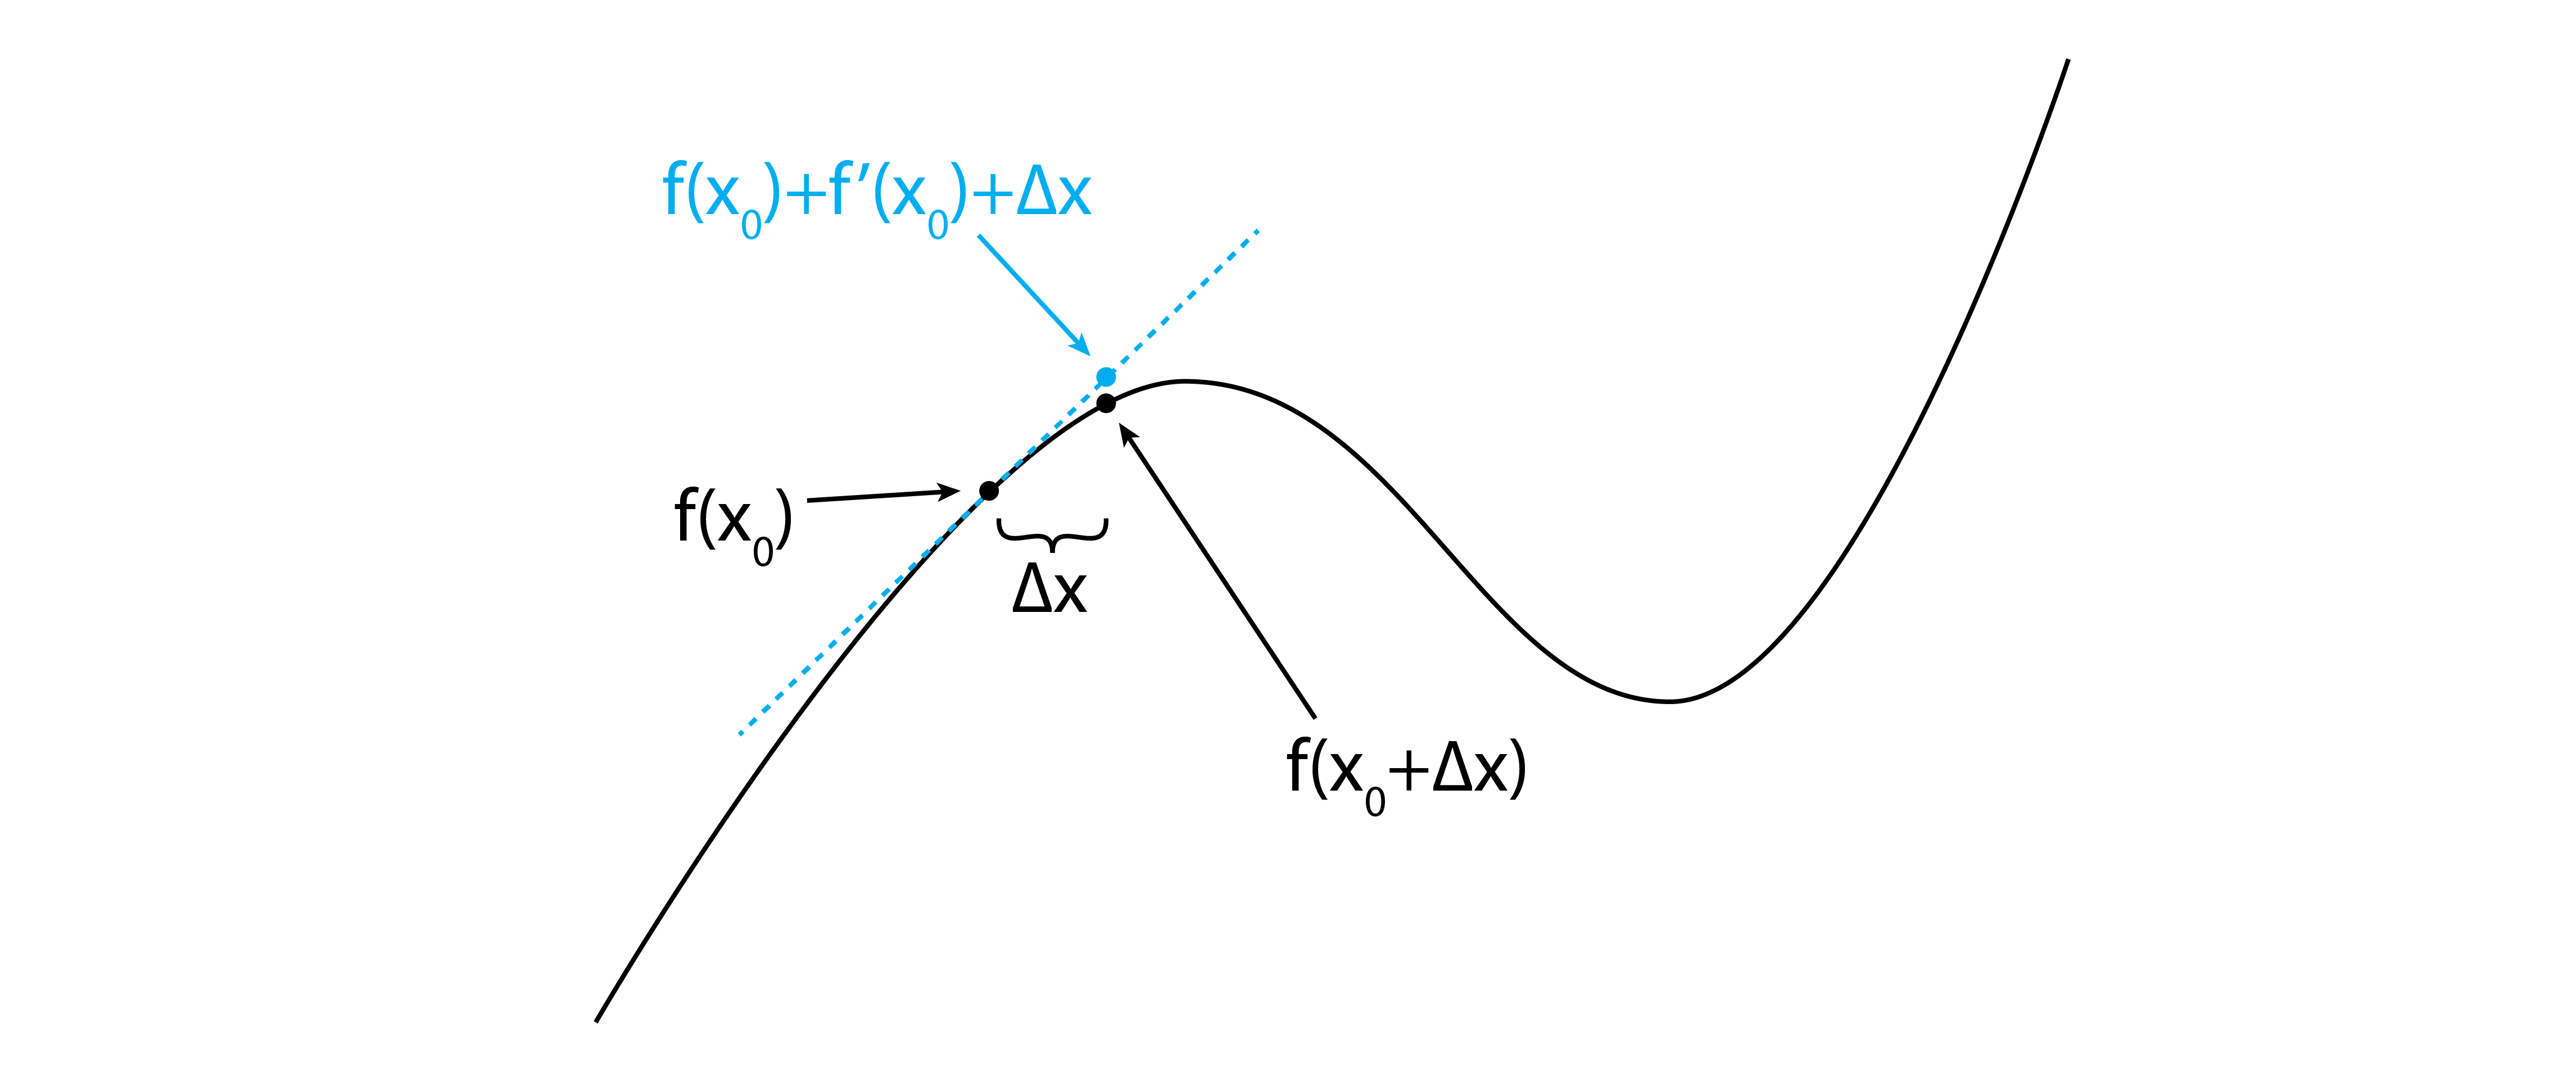
\includegraphics[width=\linewidth]{SimMethodsFDMApprox}
  \caption{Illustration of equation \ref{eq:1degTaylorApprox}, first order approximation of $f(x)$.}
  \label{fig:FDMSlopeApprox}
\end{figure}

 \begin{equation}\label{eq:fdaForward}
 f'(x_{0}) \approx \frac{f(x_{0} + \Delta  x) - f(x_{0})}{\Delta  x}
  \end{equation}
    \\
Similarly, we can evaluate the first order Taylor approximation for $\Delta x$ in the negative direction:

     \begin{equation}
 f(x_{0} - \Delta  x) \approx f(x_{0}) - f'(x_{0})\Delta x
  \end{equation}
    \\
  Rearranging this gives us an alternate form of $ f'(x_{0})$ from equation \ref{eq:fdaForward}:

 \begin{equation}\label{eq:fdaBackward}
 f'(x_{0}) \approx \frac{f(x_{0}) - f(x_{0} - \Delta  x)}{\Delta  x}
  \end{equation}
    \\
Summing equations \ref{eq:fdaForward} and \ref{eq:fdaBackward} gives yet another form:
  
     \begin{equation}\label{eq:fdaCentered}
 f'(x_{0}) \approx \frac{f(x_{0} + \Delta  x) - f(x_{0} - \Delta  x)}{2\Delta x}
  \end{equation}
  \\
  Equations \ref{eq:fdaForward}, \ref{eq:fdaBackward}, \ref{eq:fdaCentered} are referred to as the first order \textit{forward}, \textit{backward}, and \textit{centered} finite difference approximations.  We can use these as approximations to first order derivatives in a PDE so that the PDE can be rewritten in a form that is easy to solve.
  
%\subsection{Examples of First Order FDM}
%
%We can now rewrite any first order PDE using one of the first order finite difference approximations we just found.  To start, I've rewritten the 1D advection equation (\ref{eq:advection1d}) using the forward finite difference approximation (\ref{eq:fdaForward}) to approximate $\frac{\partial \psi}{\partial t}$ and the centered finite difference approximation (\ref{eq:fdaCentered}) to approximate $\frac{\partial \psi}{\partial x}$:
%
% \begin{equation}
%  \frac{ \psi(t_{0} + \Delta  t,  x_{0}) - \psi(t_{0}, x_{0})}{\Delta t} = -v_{x}\frac{\psi(t_{0}, x_{0} + \Delta  x)-\psi(t_{0}, x_{0}-\Delta x)}{2\Delta  x}
%  \end{equation}
%  \\
%  (assume $v_{x}$ is constant)\\
%  
%  Reorganizing this equation gives $\psi(t_{0}+\Delta t)$ in terms of $\psi(t_{0})$:
%  
%   \begin{equation}\label{eq:advection1Dapprox}
%  \psi(t_{0} + \Delta  t,  x_{0}) = \psi(t_{0}, x_{0})-v_{x}\Delta t \frac{\psi(t_{0}, x_{0} + \Delta  x)-\psi(t_{0}, x_{0}-\Delta x)}{2\Delta  x}
%  \end{equation}
%\\
%Assuming we know the current state of a given differential element, $\psi(t_{0}, x_{0})$, and the current state of its neighbors, $\psi(t_{0}, x_{0}+\Delta x)$ and $\psi(t_{0}, x_{0}-\Delta x)$, we can solve for the next state, $\psi(t_{0}+\Delta t, x_{0})$ (fig \ref{fig:SimMethodsFDM1D}).\\
%
%\begin{figure}
%  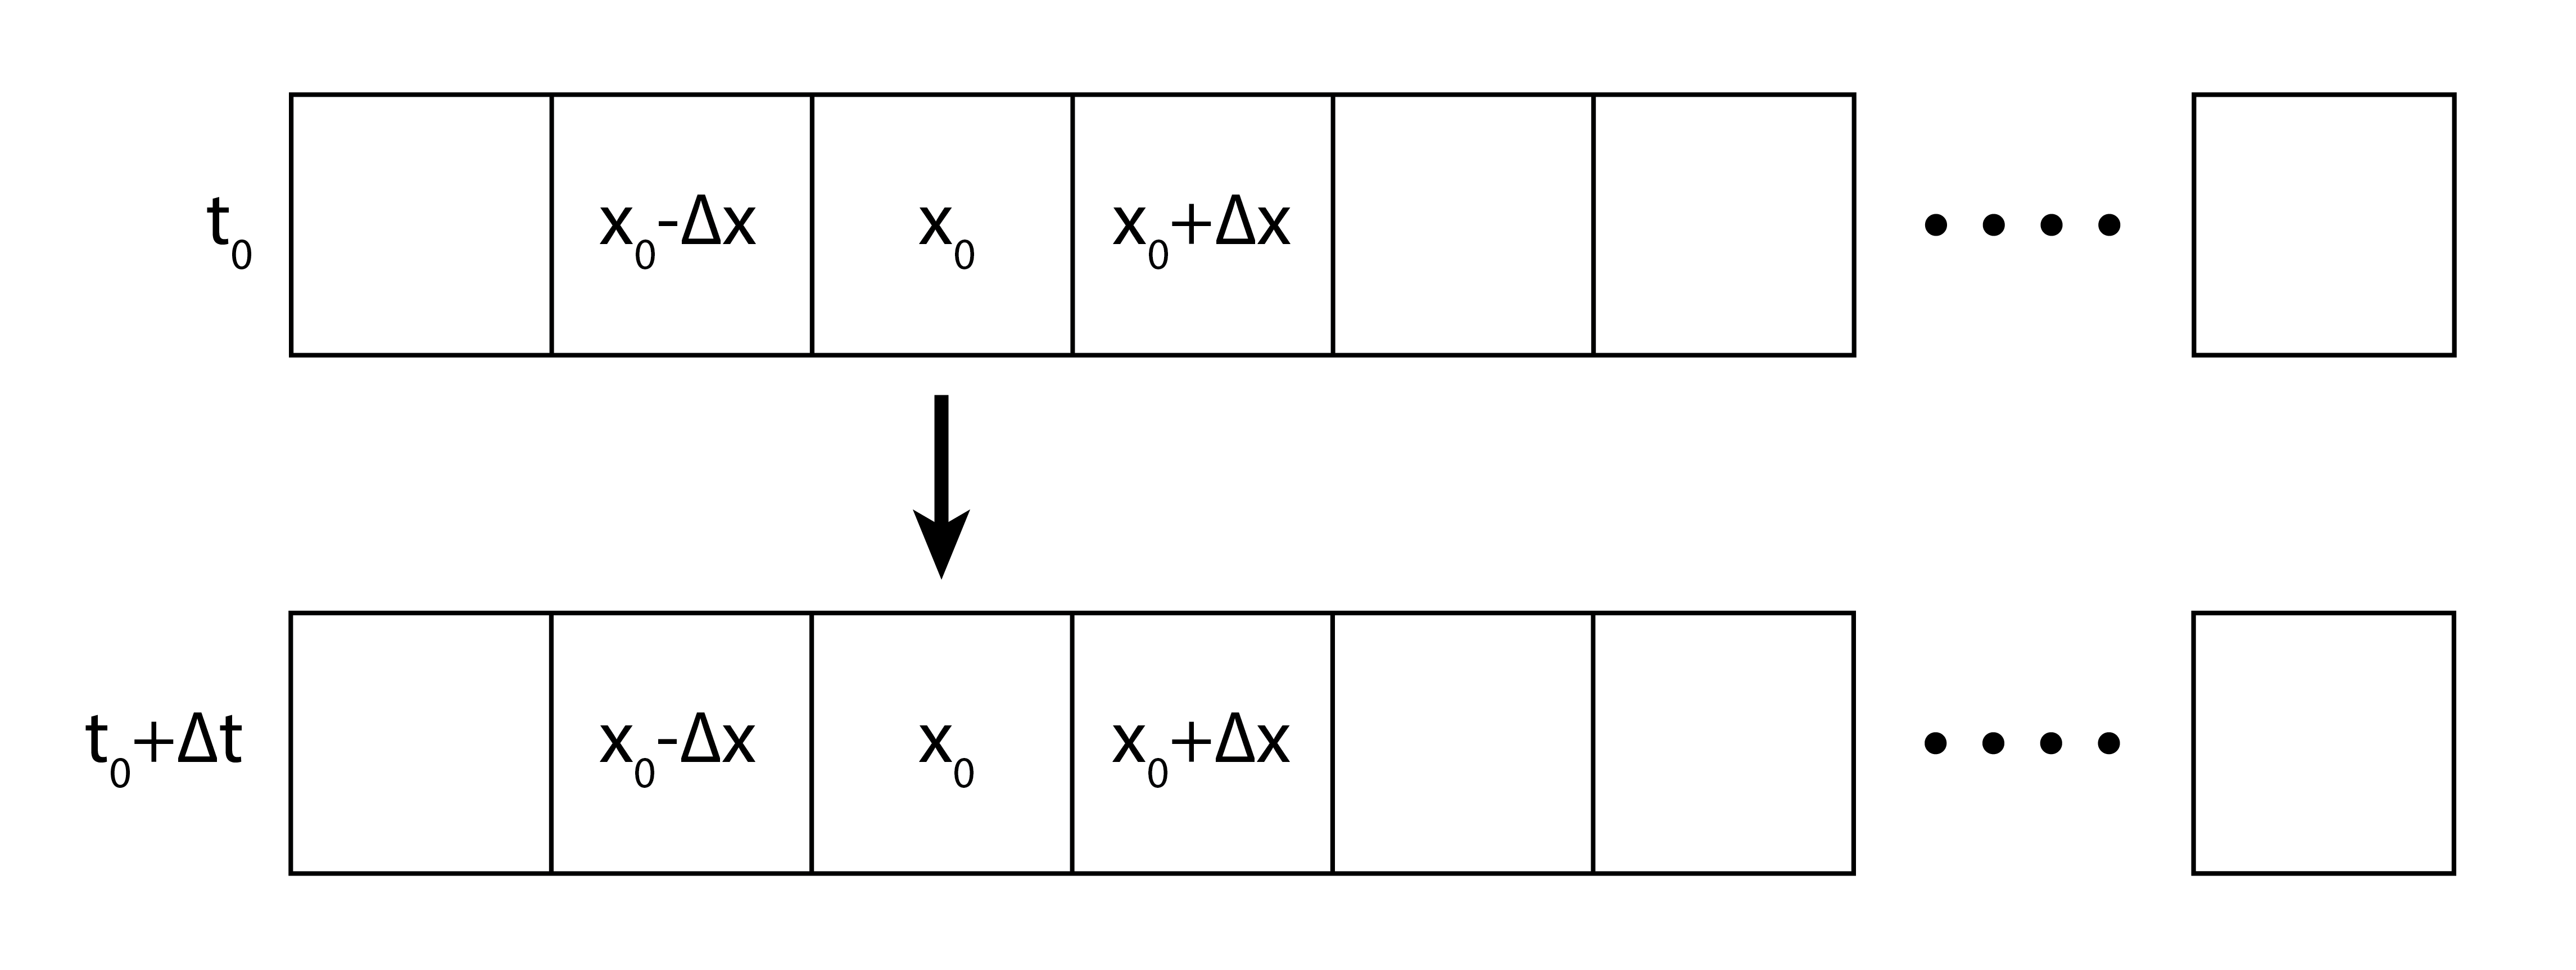
\includegraphics[width=\linewidth]{SimMethodsFDM1D.png}
%  \caption{Neighboring elements around some element at $x_{0}$ in a 1D FDM at timesteps $t_{0}$ and $t_{0}+\Delta t$.}
%  \label{fig:SimMethodsFDM1D}
%\end{figure}
%
%Similarly, we can use the backward finite difference approximation (\ref{eq:fdaBackward}) to approximate $\frac{\partial \psi}{\partial t}$ to get an equation describing the past state of the differential element $\psi(t_{0}-\Delta t, x_{0})$ in terms of its current state and the current states of its neighbors:
%
%  \begin{equation}
%  \psi(t_{0} - \Delta  t,  x_{0}) = \psi(t_{0}, x_{0}) + v_{x}\Delta t \frac{\psi(t_{0}, x_{0} + \Delta  x)-\psi(t_{0}, x_{0}-\Delta x)}{2\Delta  x}
%  \end{equation}
%  \\
%  We could reorganize this equation to solve for the forward time solution by substituting $t_{0}$ with $t_{0}+\Delta t$ and $t_{0}-\Delta t$ with $t_{0}$:
%  
%  \begin{equation}
%  \psi(t_{0},  x_{0}) = \psi(t_{0}+\Delta t, x_{0}) + v_{x}\Delta t \frac{\psi(t_{0}+\Delta, x_{0} + \Delta  x)-\psi(t_{0}+\Delta, x_{0}-\Delta x)}{2\Delta  x}
%  \end{equation}
%  \\
%  This is referred to as the \textit{implicit} method (as opposed to the \textit{explicit} method).  Implicit FDM is computationally more challenging to solve because they require solving a system of equations, rather that evaluating a single expression, however, they tend to form more stable solutions.\\
%  
%  In general, it's best to use the center finite difference approximation (\ref{eq:fdaCentered}) when you can because it has lower error than the forward or backward forms (explained more in section \ref{sec:errorAnalysis}).  If we use the center finite difference approximation for $\frac{\partial \psi}{\partial t}$, we end up with $\psi(t_{0}+\Delta t)$ as a function of $\psi(t_{0})$ and $\psi(t_{0}-\Delta t)$:
%  
%     \begin{equation}
%  \psi(t_{0} + \Delta  t,  x_{0}) = \psi(t_{0}-\Delta t, x_{0}) -v_{x}\Delta t \frac{\psi(t_{0}, x_{0} + \Delta  x)-\psi(t_{0}, x_{0}-\Delta x)}{\Delta  x}
%  \end{equation}
%  \\
%  which may or may not be possible to solve, depending on the information available.\\
%  
%  From here we can solve more complicated first order PDEs, here's an approximation of the 2D advection equation (\ref{eq:advection2d}) using a forward approximation in time and a center approximation for $x$ and $y$.  Figure \ref{fig:SimMethodsFDM2D} shows the neighboring elements in a 2D FDM.
%  
%\begin{multline}
%   \frac{ \psi(t_{0} + \Delta  t,  x_{0}, y_{0}) - \psi(t_{0}, x_{0}, y_{0})}{\Delta t} = \\
%   -v_{x}\frac{\psi(t_{0}, x_{0} + \Delta  x, y_{0})-\psi(t_{0}, x_{0}-\Delta x, y_{0})}{2\Delta  x}\\
%   -v_{y}\frac{\psi(t_{0}, x_{0}, y_{0} + \Delta  y)-\psi(t_{0}, x_{0}, y_{0}-\Delta y)}{2\Delta  y}
%\end{multline}
%
%\begin{multline}\label{eq:advection2Dapprox}
%   \psi(t_{0} + \Delta  t,  x_{0}, y_{0}) =\\
%   \psi(t_{0}, x_{0}, y_{0}) -v_{x}\Delta t\frac{\psi(t_{0}, x_{0} + \Delta  x, y_{0})-\psi(t_{0}, x_{0}-\Delta x, y_{0})}{2\Delta  x}\\
%   -v_{y}\Delta t\frac{\psi(t_{0}, x_{0}, y_{0} + \Delta  y)-\psi(t_{0}, x_{0}, y_{0}-\Delta y)}{2\Delta  y} 
%\end{multline}
%\\
%\begin{figure}
%  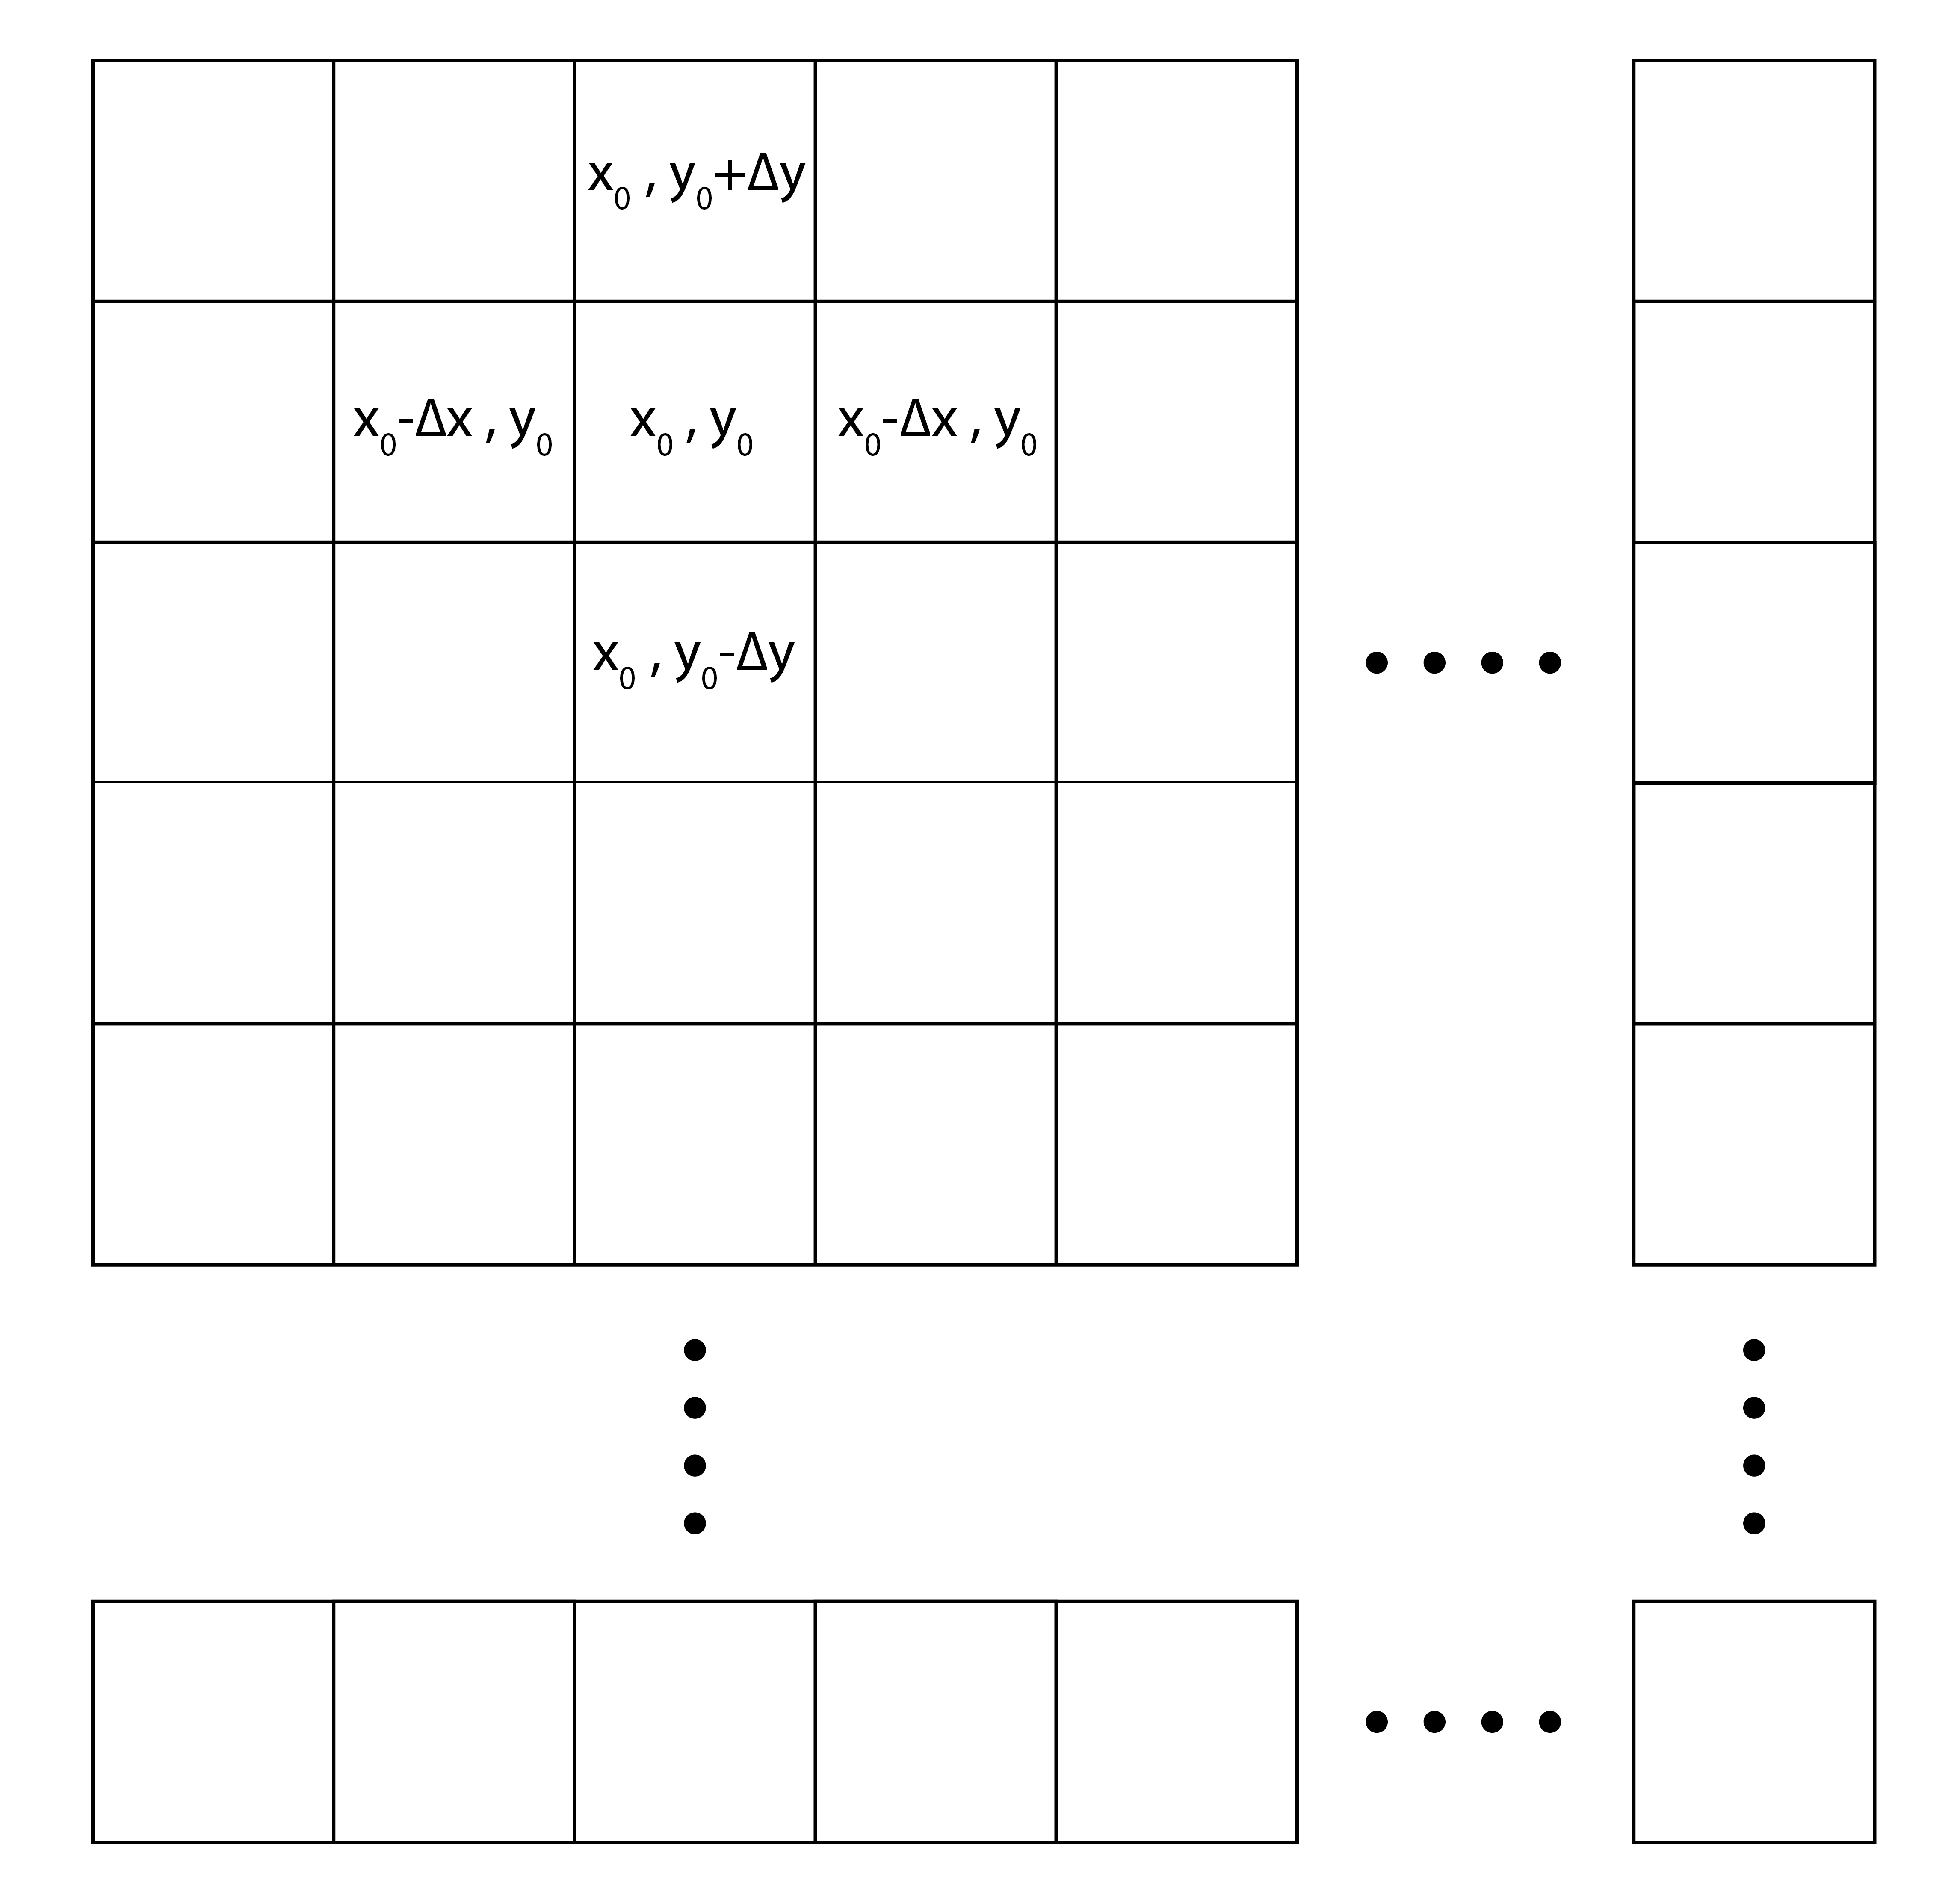
\includegraphics[width=\linewidth]{SimMethodsFDM2D.png}
%  \caption{Neighboring elements around some element at $x_{0}$, $y_{0}$ in a 2D FDM.}
%  \label{fig:SimMethodsFDM2D}
%\end{figure}
%
%\subsection{Higher Order FDM}
%
%In order to solve a second order PDE like the wave equation (\ref{eq:waveEq}), we'll need a finite difference approximation for second derivatives.  We found the first order finite difference approximations by rearranging the first order Taylor approximation (\ref{eq:1degTaylorApprox}); this time, we'll start with a second order Taylor expansion of the full Taylor Series (\ref{eq:norderTaylor}):
%
% \begin{equation}
%  f(x_{0} + \Delta  x) = f(x_{0}) + f'(x_{0})\Delta  x + \frac{f''(x_{0})}{2}\Delta  x^{2} + R_{n}(x_{0})
%  \end{equation}
%    \\
%  Again, for small $\Delta  x$, we can ignore the error term to get the second order Taylor approximation:
%  
%   \begin{equation}\label{eq:secOrderTaylorApprox}
%  f(x_{0} + \Delta  x) \approx f(x_{0}) + f'(x_{0})\Delta  x + \frac{f''(x_{0})}{2}\Delta  x^{2}
%  \end{equation}
%    \\
%  And similarly for  $f(x_{0} - \Delta  x)$:
%  
%     \begin{equation}\label{eq:secOrderTaylorApproxNeg}
%  f(x_{0} - \Delta  x) \approx f(x_{0}) - f'(x_{0})\Delta  x + \frac{f''(x_{0})}{2}\Delta  x^{2}
%  \end{equation}
%    \\
%  Adding equations \ref{eq:secOrderTaylorApprox} and \ref{eq:secOrderTaylorApproxNeg} cancels out the $f'(x_{0})$ terms:
%  
%   \begin{equation}
%  f(x_{0} + \Delta  x) + f(x_{0} - \Delta  x) \approx 2f(x_{0}) + f''(x_{0})\Delta  x^{2}
%  \end{equation}
%    \\
%  Rearranging gives us the centered second order finite differential approximation:
%  
%   \begin{equation}\label{eq:fdaseccentered}
%   f''(x_{0}) \approx \frac{f(x_{0} + \Delta  x) - 2f(x_{0}) + f'(x_{0} -\Delta  x)}{\Delta  x^{2}}
%  \end{equation}
%    \\
%  The forward second order finite differential approximation requires equation \ref{eq:secOrderTaylorApprox} and an approximation of $f'(x_{0} + 2\Delta  x)$:
%  
%  \begin{equation}\label{eq:secOrderTaylorApprox2}
%  f(x_{0} + 2\Delta  x) \approx f(x_{0}) + f'(x_{0})2\Delta  x + \frac{f''(x_{0})}{2}4\Delta  x^{2}
%  \end{equation}
%    \\
%  Subtracting 2x equation \ref{eq:secOrderTaylorApprox} from \ref{eq:secOrderTaylorApprox2} gives:
%  
%    \begin{equation}
%  f(x_{0} + 2\Delta  x) - 2f(x_{0} + \Delta  x) \approx -f(x_{0}) + f''(x_{0})\Delta  x^{2}
%  \end{equation}
%  \\
%Which simplifies to the forward second order finite differential approximation:
%  
%      \begin{equation}\label{eq:fdasecforward}
%f''(x_{0}) \approx \frac{f(x_{0} + 2\Delta  x) - 2f(x_{0} + \Delta  x) + f(x_{0})}{\Delta  x^{2}}
%  \end{equation}
%  \\
%  The backward second order finite differential approximation is calculated similarly:
%  
%        \begin{equation}\label{eq:fdasecbackward}
%f''(x_{0}) \approx \frac{f(x_{0} - 2\Delta  x) - 2f(x_{0} - \Delta  x) + f(x_{0})}{\Delta  x^{2}}
%  \end{equation}
%  \\
% Beyond this, higher order finite differential approximations may be calculated similarly, or from the following general forms of the forward (\ref{eq:generalFDAForward}), backward (\ref{eq:generalFDABackward}), and center (\ref{eq:generalFDACenter}) $n$th order finite difference approximations:
% 
%  \begin{equation}\label{eq:generalFDAForward}
% f^{n}(x_{0}) \approx \frac{1}{\Delta  x^{n}}\sum_{i=0}^{n}(-1)^{i}\binom {n} {i}f(x_{0} + (n-i)\Delta  x)
% \end{equation}
% 
% \begin{equation}\label{eq:generalFDABackward}
% f^{n}(x_{0}) \approx \frac{1}{\Delta  x^{n}}\sum_{i=0}^{n}(-1)^{i}\binom {n} {i}f(x_{0} - i\Delta  x)
% \end{equation}
% 
%  \begin{equation}\label{eq:generalFDACenter}
% f^{n}(x_{0}) \approx \frac{1}{\Delta  x^{n}}\sum_{i=0}^{n}(-1)^{i}\binom {n} {i}f(x_{0} + \left(\frac{n}{2}-i\right)\Delta  x)
% \end{equation}
% 
%\subsection{Examples of Second Order FDM}\label{sec:secondOrderExamples}
%
%Now that we have a second order finite difference approximation, we can solve second order PDEs numerically with FDM.  The 1D heat equation (\ref{eq:heat1d}) can be approximated using the first order forward approximation (\ref{eq:fdaForward}) for $\frac{\partial T}{\partial t}$ and the second order center approximation (\ref{eq:fdaseccentered}) for $\frac{\partial^{2} T}{\partial x^{2}}$:\\
%
% \begin{equation}
%  \frac{T(t_{0} + \Delta  t, x_{0}) - T(t_{0}, x_{0})}{\Delta  t} = c\frac{T(t_{0},x_{0} + \Delta  x)- 2T(t_{0},x_{0}) + T(t_{0},x_{0} -\Delta  x)}{\Delta  x^{2}}
%  \end{equation}
%\\
% \begin{equation}\label{eq:heatfda1D}
%  T(t_{0} + \Delta  t, x_{0}) = T(t_{0}, x_{0}) + c\Delta  t\frac{T(t_{0},x_{0} + \Delta  x) - 2T(t_{0},x_{0}) + T(t_{0},x_{0} -\Delta  x)}{\Delta  x^{2}}
%  \end{equation}
%\\
%Similarly, the 2D wave equation \ref{eq:wave2d} is approximated with the second order center approximation (\ref{eq:fdaseccentered}) for $\frac{\partial^{2} u}{\partial x^{2}}$, $\frac{\partial^{2} u}{\partial y^{2}}$ and $\frac{\partial^{2} u}{\partial t^{2}}$:
%
% \begin{multline}
%\frac{u(t_{0} + \Delta  t,x_{0},y_{0})- 2u(t_{0},x_{0},y_{0}) + u(t_{0} -\Delta  t,x_{0},y_{0})}{\Delta  t^{2}} = \\
%c\frac{u(t_{0},x_{0} + \Delta  x,y_{0})- 2u(t_{0},x_{0},y_{0}) + u(t_{0},x_{0} -\Delta  x,y_{0})}{\Delta  x^{2}}\\
%+c\frac{u(t_{0},x_{0},y_{0}+ \Delta  y)- 2u(t_{0},x_{0},y_{0}) + u(t_{0},x_{0},y_{0} -\Delta  y)}{\Delta  y^{2}}
%  \end{multline}
%  
%   \begin{multline}\label{eq:wavefda2d}
%u(t_{0} + \Delta  t,x_{0},y_{0})  = 2u(t_{0},x_{0},y_{0})-u(t_{0} -\Delta  t,x_{0},y_{0})\\
%+c\Delta  t^{2}\frac{u(t_{0},x_{0} + \Delta  x,y_{0})- 2u(t_{0},x_{0},y_{0}) + u(t_{0},x_{0} -\Delta  x,y_{0})}{\Delta  x^{2}}\\
%+c\Delta  t^{2}\frac{u(t_{0},x_{0},y_{0}+ \Delta  y)- 2u(t_{0},x_{0},y_{0}) + u(t_{0},x_{0},y_{0} -\Delta  y)}{\Delta  y^{2}}
%  \end{multline}
%\\
%Since the wave equation contains a second order partial derivative with respect to t, the next time step $u(t_{0} + \Delta  t,x_{0},y_{0})$ must depend on both the current $u(t_{0},x_{0},y_{0})$ and previous $u(t_{0}-\Delta t,x_{0},y_{0})$ time steps in the equation above.
%
%\subsection{Boundary Conditions}
%
%Suppose some element lives at the left edge of the region we are evaluating with a center finite difference approximation; it will not a have a neighbor to its left ($x_{0}-\Delta x$).  This situation is illustrated in Figure \ref{fig:FDMBoundary}.  In this case, we need to decide how to process an element at the boundary, called a \textit{boundary condition}.\\
%
%\begin{figure}
%  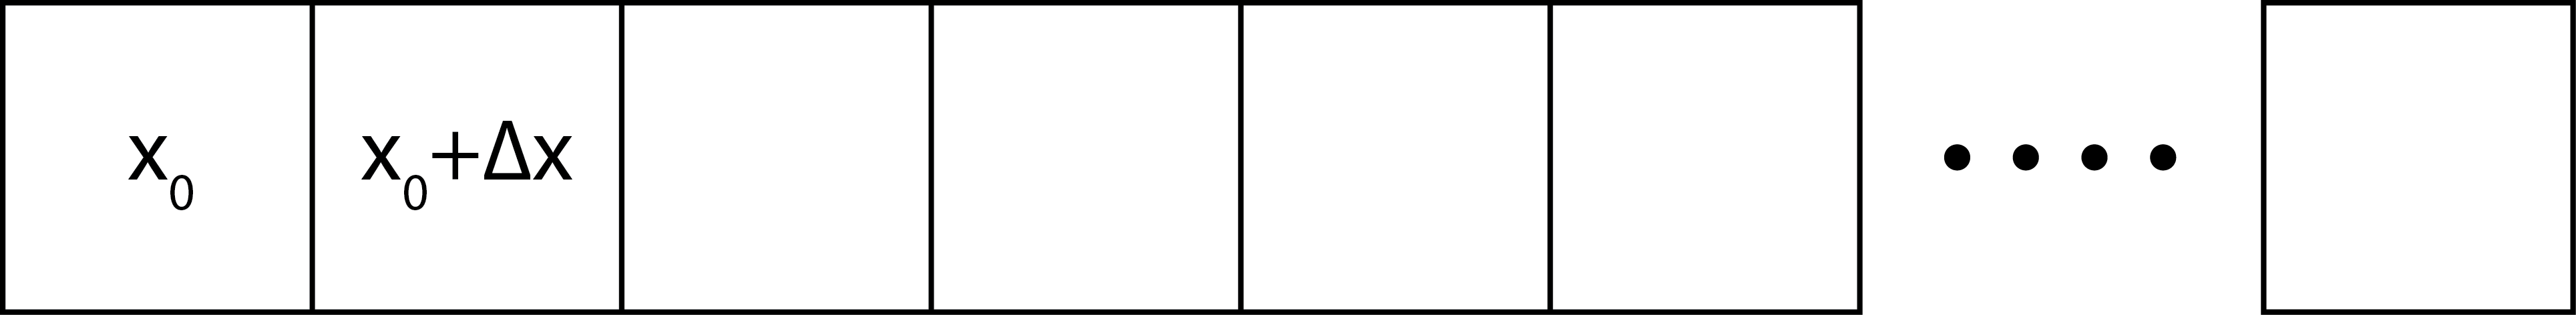
\includegraphics[width=\linewidth]{SimMethodsFDMBoundary.png}
%  \caption{Element at the boundary of a 1D FDM has no neighbor at $x_{0}-\Delta x$.}
%  \label{fig:FDMBoundary}
%\end{figure}
%
%One option is to use a forward finite difference approximation for this cell (\ref{eq:fdaForward}), since it only depends on $x_{0}$ and $x_{0}+\Delta x$.  
%
%\subsection{Example Code}
%
%\begin{figure}
%  \includegraphics[width=\linewidth]{reactionDiffusion.png}
%  \caption{Time sequence showing the abundance of chemical v in a Gray-Scott reaction across 2D space for 9 time steps.  Each pixel represents one finite element.  System is initialized with a random patch of chemicals u and v at t = 0 and then solved for with the following parameters: $F = 0.0545$, $k=0.062$.  Live, interactive demo available at \href{http://git.amandaghassaei.com/ReactionDiffusionShader/}{Github}.}
%  \label{fig:grayScott}
%\end{figure}
%
%A popular pair of PDEs are the Gray-Scott \href{https://en.wikipedia.org/wiki/Reaction%E2%80%93diffusion_system#Two-component_reaction.E2.80.93diffusion_equations}{Reaction-Diffusion} equations.  These equations describe the interactions between two chemicals, u and v, as they react with each other and diffuse across space:
%
% \begin{equation}\label{eq:gs1}
%  \frac{\partial u}{\partial t} = D_{u}\nabla^{2} u -uv^{2} + F(1-u)
%  \end{equation}
%  
%   \begin{equation}\label{eq:gs2}
%  \frac{\partial v}{\partial t} = D_{v}\nabla^{2} v +uv^{2} - (F+k)v
%  \end{equation}
%  
%  where $t$ is time, $u$ and $v$ are the concentrations of chemicals u and v, $D_{u}$ and $D_{v}$ are the rates of diffusion for chemicals u and v, and $F$ and $k$ are additional constants.  \\
%  
%  Equation \ref{eq:gs1} tells us how quickly the abundance of chemical u is changing and equation \ref{eq:gs2} tells us how quickly the abundance of chemical v is changing.  The first terms of both equations describe the rate of diffusion of each chemical across the spatial dimensions.  The second terms describe the reaction between chemicals u and v.  We can see that the reaction between u and v depletes chemical u and generates chemical v from the sign of these second terms.  The positive third term in equation \ref{eq:gs1} represents the replenishment of chemical u in the system; without this term, u would quickly become depleted through reactions with v.  The negative third term in equation \ref{eq:gs2} represents the diminishment of chemical v, proportional to the concentration of v; without this term v would grow uncontrollably due to reactions with u.\\
%  
%  A plot of a 2D Gray-Scott system (Fig \ref{fig:grayScott}) shows the concentration or chemical v over time.  I wrote an interactive demo of this system using GPU shaders that is live at  \href{http://git.amandaghassaei.com/ReactionDiffusionShader/}{Github}.  In my demo, clicking on the screen introduces more of chemical v into the system.\\
%  
%  Consider the 2D Gray Scott PDEs:
%  
%   \begin{equation}
%  \frac{\partial u}{\partial t} = D_{u}\left(\frac{\partial^{2} u}{\partial x^{2}}+\frac{\partial^{2} u}{\partial y^{2}} \right) -uv^{2} + F(1-u)
%  \end{equation}
%  
%   \begin{equation}
%  \frac{\partial v}{\partial t} = D_{v}\left(\frac{\partial^{2} v}{\partial x^{2}}+\frac{\partial^{2} v}{\partial y^{2}} \right) +uv^{2} - (F+k)v
%  \end{equation}
%  \\
%  Following the steps outlined in section \ref{sec:secondOrderExamples}, we'll approximate these PDEs using finite difference approximations.  By applying the first order forward approximation (\ref{eq:fdaForward}) to $\frac{\partial u}{\partial t}$ and $\frac{\partial v}{\partial t}$ and second order center approximations (\ref{eq:fdaseccentered}) to $\frac{\partial^{2} u}{\partial x^{2}}$, $\frac{\partial^{2} u}{\partial y^{2}}$, $\frac{\partial^{2} v}{\partial x^{2}}$, and $\frac{\partial^{2} v}{\partial y^{2}}$, we get a expressions for $u(t_{0} + \Delta  t, x_{0}, y_{0})$ and $v(t_{0} + \Delta  t, x_{0}, y_{0})$:
%  
%   \begin{multline}\label{eq:gsdifferentialu}
%    u(t_{0} + \Delta  t, x_{0}, y_{0}) = \Delta  t[-u(t_{0}, x_{0}, y_{0})v(t_{0}, x_{0}, y_{0})^{2} - (F+k)v(t_{0}, x_{0}, y_{0})] + u(t_{0}, x_{0}, y_{0})\\
%    + D_{u}\Delta  t\frac{u(t_{0},x_{0} + \Delta  x, y_{0})- 2u(t_{0},x_{0}, y_{0}) + u(t_{0},x_{0} -\Delta  x, y_{0})}{\Delta  x^{2}} \\
%    + D_{u}\Delta  t\frac{u(t_{0},x_{0} , y_{0}+ \Delta  y)- 2u(t_{0},x_{0}, y_{0}) + u(t_{0},x_{0} , y_{0}-\Delta  y)}{\Delta  y^{2}}
%  \end{multline}
%  
%    \begin{multline}\label{eq:gsdifferentialv}
%    v(t_{0} + \Delta  t, x_{0}, y_{0}) = \Delta  t[u(t_{0}, x_{0}, y_{0})v(t_{0}, x_{0}, y_{0})^{2} + F(1-u(t_{0}, x_{0}, y_{0}))] + v(t_{0}, x_{0}, y_{0})\\
%    + D_{v}\Delta  t\frac{v(t_{0},x_{0} + \Delta  x, y_{0})- 2v(t_{0},x_{0}, y_{0}) + v(t_{0},x_{0} -\Delta  x, y_{0})}{\Delta  x^{2}} \\
%    + D_{v}\Delta  t\frac{v(t_{0},x_{0} , y_{0}+ \Delta  y)- 2v(t_{0},x_{0}, y_{0}) + v(t_{0},x_{0} , y_{0}-\Delta  y)}{\Delta  y^{2}}
%  \end{multline}
%  \\
%  To implement this system on a computer, start with the following Javascript code:
%
%\begin{lstlisting}[language=JavaScript]
%//u is a 2D array with dimensions xMax, yMax
%//v is a 2D array with dimensions xMax, yMax
%//nextU is a 2D array with dimensions xMax, yMax
%//nextV is a 2D array with dimensions xMax, yMax
%//constants: Du, Dv, F, k, deltaT, deltaX, deltaY
%
%while (true){ //repeat forever
%	
%    for (var x=0; x < xMax; x++){
%    	for (var y=0; y < yMax; y++){
%    	
%	    //current state
%	    var currentU = u[x][y];
%	    var currentV = v[x][y];
%		
%	    //neighbor states
%	    var currentUplusX = u[x+1][y];
%	    var currentUplusX = u[x-1][y];
%	    var currentVplusY = u[x][y+1];
%	    var currentVminusY = u[x][y-1];
%		
%		
%	    //lagrangian approximations
%	    var lagrangianU = (currentUplusX-2*currentU+currentUminusX)/(deltaX*deltaX) 
%		+ (currentUplusY-2*currentU+currentUminusY)/(deltaY*deltaY); 
%			
%	    var lagrangianV = (currentVplusX-2*currentV+currentVminusX)/(deltaX*deltaX)
%		+ (currentVplusY-2*currentV+currentVminusY)/(deltaY*deltaY); 
%		
%		
%	    nextU[x][y] = deltaT*(-currentU*currentV*currentV-(F + k)*currentV) 
%		+ currentU + Du*deltaT*lagrangianU;
%			
%	    nextV[x][y] = deltaT*(currentU*currentV*currentV+F*(1 - currentU)) 
%		+ currentV + Dv*deltaT*lagrangianV;
%    	}
%    }
%    
%    u = nextU;
%    v = nextV;
%}
%\end{lstlisting}
%
%
%Next, we must decide how to handle the boundary conditions, for now set the boundaries equal to 1 in the u array and 0 in the v array:
%
%\begin{lstlisting}[language=JavaScript]
%....
%
%while (true){ //repeat forever
%	
%    for (var x=0; x < xMax; x++){
%    	for (var y=0; y < yMax; y++){
%    	
%	    //current state
%	    var currentU = u[x][y];
%	    var currentV = v[x][y];
%		
%	    //neighbor states
%	    var currentUplusX;
%	    if (x == xMax-1) currentUplusX = 0;
%	    else currentUplusX = u[x+1][y];
%	    
%	    var currentUminusX;
%	    if (x == 0) currentUminusX = 0;
%	    else currentUminusX = u[x-1][y];
%	    
%	    var currentUplusY;
%	    if (y == yMax-1) currentUplusY = 1;
%	    else currentUplusY = u[x][y+1];
%	    
%	    var currentUminusY;
%	    if (y == 0) currentUminusY = 1;
%	    else currentUminusY = u[x][y-1];
%		
%	    ....
%	
%    	}
%    }
%    
%    ....
%    
%}
%\end{lstlisting}
%
%Finally, we must set the initial conditions and constants:\\
%\begin{lstlisting}[language=JavaScript]
%var Du = 0.2;
%var Dv = 0.1;
%var F = 0.0545;
%var k = 0.062;
%var deltaT = 1;
%var deltaX = 1;
%var deltaY = 1;
%
%var xMax = 100;
%var yMax = 100;
%
%var u = initEmptyArray();
%var v = initEmptyArray();
%var nextU = initEmptyArray();
%var nextV = initEmptyArray();
%
%function initEmptyArray(){//javascript does not do this particularly gracefully
%    var array = [];
%    for (var x=0; x < xMax; x++){
%    	var column = [];
%	for (var y=0; y < yMax; y++){
%	    column.push(0);
%	}
%	array.push(column);
%    }
%    return array;
%}
%
%//set initial values in a center patch of the u and v arrays
%var patchSize = 10;
%for (var x=0; x < xMax; x++){
%    for (var y=0; y < yMax; y++){
%	if ((x > xMax/2 - patchSize) && (x < xMax/2 + patchSize) 
%	    && (y > yMax/2 - patchSize) && (y < yMax/2 + patchSize)) {
%	    //inside center patch
%	    u[x][y] = 0.5 + Math.random()*0.02 - 0.01;
%	    v[x][y] = 0.25 + Math.random()*0.2 - 0.01;
%	} else {
%	    //set u = 1 and v = 0 everywhere else
%	    u[x][y] = 1;
%	    v[x][y] = 0;
%	}
%    }
%}
%
%....
%
%\end{lstlisting}
%
%Plotting out v over time gives the images shown in Fig \ref{fig:grayScott}.  Changing the constants in the PDEs, especially F and k, will yield reaction diffusion behavior that varies wildly.  Further exploration of the Gray-Scott parameters is given by Munafro\cite{Munafo2016}.
%
%\subsection{Error Analysis}\label{sec:errorAnalysis}
%
% \begin{equation}
% f'(x_{0}) = \frac{f(x_{0} + \Delta  x) - f(x_{0})}{\Delta  x} + \frac{R_{1}(x_{0})}{\Delta  x}
%  \end{equation}
%  
%For small changes $\Delta  x$ in the negative direction, equation  can be rearranged to:
%
% \begin{equation}
% f'(x_{0}) = \frac{f(x_{0}) - f(x_{0} - \Delta  x)}{\Delta  x} - \frac{R_{1}(x_{0})}{\Delta  x}
%  \end{equation}
%  
%  fjalsdjflkadsjf
%  
%   \begin{equation}
% f'(x_{0}) = \frac{f(x_{0} + \Delta  x) - f(x_{0} - \Delta  x)}{2\Delta x} + \frac{R_{1}(x_{0})}{2\Delta  x}
%  \end{equation}
%  
%  Finally, since these computations will more likely be happening inside a computer, it's important to take note of the aggregation of float precision error in the calculations.  Even with increasingly small $\Delta t$ and $\Delta x$, numerical results calculated on a computer will never perfectly match the exact values due to these floating point errors.
%  
%  \subsection{Decreasing FDM Error}
%  
%  \subsubsection{Relationship to Other Numerical Integration Techniques}
%  
%  \href{https://en.wikipedia.org/wiki/Euler_method}{Euler integration} is a simple numerical technique for solving differential equations that is based on the first order forward and backward finite difference approximations (\ref{eq:fdaForward} and \ref{eq:fdaBackward}).  The \href{https://en.wikipedia.org/wiki/Midpoint_method}{midpoint method} is a modification to Euler integration based on the center finite difference approximation (\ref{eq:fdaCentered}).  Euler integration and the midpoint method are the simplest forms of the \href{https://en.wikipedia.org/wiki/Runge%E2%80%93Kutta_methods}{Runge-Kutta method}.\\
%
%Lagrangian polynomial interpolation
%    
%  \subsection{FDM as a Cellular Automaton Ruleset}
%
%A \href{https://en.wikipedia.org/wiki/Cellular_automaton}{cellular automaton} (CA) is a discretized model used to describe the dynamics of a system.  CAs are discrete in both space in time, meaning space is divided up into many identical \textit{cells} and time moves forward in discrete \textit{steps}.  Each cell owns one or many state variables, which may hold binary or continuous data.  The governing equations of a CA system are codified in the \textit{ruleset} that applies universally across all cells in the system; typically a ruleset describes local interactions of a cell with its neighbors.  For example, in the popular CA \href{https://en.wikipedia.org/wiki/Conway's_Game_of_Life}{Conway's Game of Life}, the state of a 2D cell in the next time step is a function of its current state and the state of its eight neighbors.\\
%
%By solving PDEs using forward finite difference approximations for partial derivates with respect to time, and centered finite difference approximations for partial derivatives with respect to spatial dimensions, we get a form of the PDE that reads like a CA ruleset.  Equations \ref{eq:advection1Dapprox}, \ref{eq:advection2Dapprox}, \ref{eq:heatfda1D}, \ref{eq:gsdifferentialu}, and \ref{eq:gsdifferentialv} have the general form: the next state of a differential element equals some function of its current state and the current state of its neighbors. CA rulesets are an explicit formulation of the FDM.\\
%
%A longer discussion of PDEs, FDM, and CAs is given in Yang et al\cite{Yang2010}
%
%\subsection{Semi-discrete FDM}
%
%We can also compute a \textit{semi-discrete} numerical solution to a PDE that is discrete in one dimension, but continuous in another.  For example, a semi-discrete FDM for the 1D heat equation (\ref{eq:heat1d}) that is continuous in time is given below:
%
% \begin{equation}
%  \frac{\partial T}{\partial t} = c\Delta  t\frac{T(t_{0},x_{0} + \Delta  x) - 2T(t_{0},x_{0}) + T(t_{0},x_{0} -\Delta  x)}{\Delta  x^{2}}
%  \end{equation}
%  \\
%  Systems with one continuous independent variable can be solved by the \href{https://en.wikipedia.org/wiki/Method_of_lines}{Method of Lines}, using well established techniques of numerical integration of initial-value problems.
  
\section{Differential vs Integral Forms}
\section{Finite Element Method}
\subsection{Catmull-Clark Subdivision}
\subsection{Octree Subdivision}
\section{Finite Volume Method}
\section{Multigrid Method}

\section{Further Reading}


